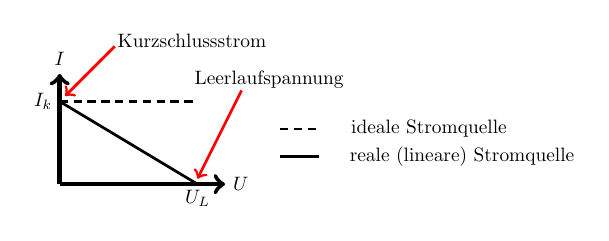
\begin{tikzpicture}[line width=1pt, scale=0.7, transform shape]
\draw [->, ultra thick] (0,0) -- (0,2) node[above]{$I$};
\draw [->, ultra thick] (0,0) -- (3,0) node[right]{$U$};
\draw [densely dashed] (0,1.5) -- (2.5,1.5);
\draw (0,1.5) -- (2.5,0);
\draw [<-, red] (0.1,1.6) -- (1,2.5);
\draw [<-, red] (2.5,0.1) -- (3.3,1.7);
\node [very thick] at (2.4,2.6) {Kurzschlussstrom};
\node [very thick] at (3.8,1.9) {Leerlaufspannung};
\node [] at (2.5, -0.25) {$U_L$};
\node [] at (-0.3,1.5) {$I_k$};

\draw [densely dashed] (4,1) -- (4.7,1);
\node [] at (6.7,1) {ideale Stromquelle};
\draw (4,0.5) -- (4.7,0.5);
\node [] at (7.3,0.5) {reale (lineare) Stromquelle};
\end{tikzpicture}